\documentclass[12pt,a4paper]{article}
\usepackage{rmpackages}																% usual packages
\usepackage{rmtemplate}																% graphic charter
\usepackage{rmexocptce}																% for DS with cptce eval
\usetikzlibrary{shapes}

\cfoot{} 													% if no page number is needed
%\renewcommand\arraystretch{1.5}		% stretch table line height

\begin{document}

\begin{header}
Mesurer une molécule -- Aides
\end{header}

\hrule{}
\vspace{5pt}
\begin{enumerate}
\item Pour son expérience, Benjamin Franklin utilise une petite cuillère à café qui contient un volume $V_\mathrm{cac}$ de liquide.
On prendra comme valeur du volume d'une telle cuillère :
\[
V_\mathrm{cac} = \unit{2{,}0}{mL}.
\]

\hrule{}
\vspace{5pt}
\item
L'aire $S$ de la tache d'huile est :
\[
S = \unit{2000}{m\squared}.
\]

\hrule{}
\vspace{5pt}
\item 
\begin{multicols}{2}
Aire $S$ d'un cercle de rayon $r$ :
\[
S = \pi r^2
\]

Attention aux unités :
\begin{itemize}
\item[•] $r$ est en mètres (m) ;
\item[•] $S$ est en mètres carrés (m\textsuperscript{2}).
\end{itemize}
\hfill

\begin{center}
\begin{tikzpicture}
\draw (0,0) circle (2) ;
\draw (0,0) -- (2,0) ;
\draw (0,0) node {$\times$} ;
\draw (1, 0) node[above]{$r$} ;
\end{tikzpicture}
\end{center}
\end{multicols}

\hrule{}
\vspace{5pt}
\item Volume $V$ d'un cylindre de section $S$ et d'épaisseur $e$ :
\begin{multicols}{2}
\[
V = S \times e
\]
Attention aux unités :
\begin{itemize}
\item[•] $e$ est en mètres (m) ;
\item[•] $S$ est en mètres carrés (m\textsuperscript{2}) ;
\item[•] $V$ est en mètres cubes (m\textsuperscript{3}).
\end{itemize}
\hfill

\hfill
\begin{center}
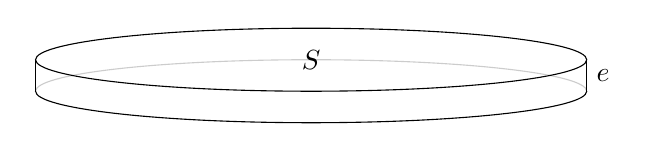
\begin{tikzpicture}
\draw (0,0) ellipse (3.5 and 0.4);
\fill[white,opacity=0.8] (-3.6,0) rectangle (3.6, 0.5);
\draw (0,0.4) ellipse (3.5 and 0.4);
\draw (0,0.4) node {$S$};
\draw (-3.5,0) -- (-3.5,0.4);
\draw (3.5,0) -- (3.5,0.4);
\draw (3.5,0.2) node[right] {$e$} ;
\end{tikzpicture}
\end{center}
\end{multicols}

\hrule{}
\vspace{5pt}
\item L'huile d'olive est composée majoritairement d'oléine, aussi appelée trioléine, dont la formule est $\oleine$.
Une molécule d'oléine est représentée ci-dessous.
Les boules grises représentent les atomes de carbone, les blanches représentent les atomes d'hydrogène et les rouges représentent les atomes d'oxygène.
\begin{center}
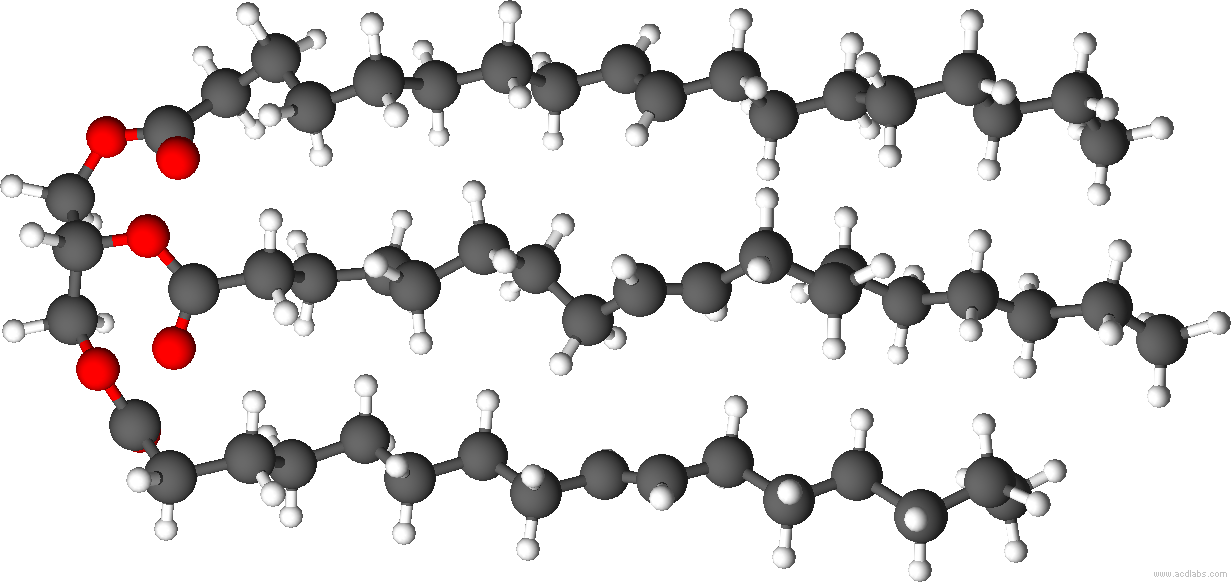
\includegraphics[scale=0.2]{images/oleine.png}
\end{center}
\hrule{}
\end{enumerate}

\end{document}